\documentclass{article}
\usepackage{civ}

\title{CIV102: Structures and Materials Notes}
\author{QiLin Xue}
\date{Fall 2020}
\usepackage{physics}
\usepackage{siunitx}
\usepackage{mathrsfs}
\usepackage{ wasysym }

\usetikzlibrary{arrows}
\begin{document}

\maketitle
\section{Lecture 1}
\begin{idea}
    The three basic principles of engineering are:
    \begin{itemize}
        \item $F=ma$
        \item You can't push on a rope.
        \item A necessary condition for solving any given engineering problem is to know the answer before starting.
    \end{itemize}
\end{idea}
\section{Inelastic Behaviour}
\begin{itemize}
    \item Permanent deformation can be defined in three ways:
    \begin{enumerate}
        \item Upon unloading, sample does not return to original dimensions
        \item Strain does not return to zero
        \item Atoms move to new positions
        \item Occurs near the end of linear behaviour
    \end{enumerate}
    \item Plastic comes from the greek word \textit{plastikos}, which means to shape or to sculpt. In this course, plastic does not refer to the material type but instead the permanent deformation.
    \item The \textbf{strength} of a material describes when the permanent deformation occurs.
    \begin{warning}
        Strength depends on context and is not always defined as above.
    \end{warning}
    \item The stress strain curve for different materials resemble different shapes.
    \begin{itemize}
        \item Polymers have a distinct yielding region
        \item Metals start a concave down behaviour as soon as elastic deformation ends
        \item Ceramics have linear behaviour all the way until they fracture
    \end{itemize}
    \begin{figure}[ht]
        \centering
        \incfig{stress_strain}
    \end{figure}
    \item For polymers, the use of \textit{Young's Modulus} is misleading since the elastic behaviour depends on several different types of bonds, while Young's Modulus is related to the bahviour of a single bond. As a result, the term \textbf{elastic modulus} is used to describe polymers and composite materials.
    \subsection{Ceramics}
    \item Ceramics are not typically tested in tension because:
    \begin{enumerate}
        \item It is difficult to grip because it crumbles easily
        \item It is difficult to shape it into a dogbone shape
        \item Machine alignment is difficult to achieve.
    \end{enumerate}
    \item Instead, we test them by \textbf{3-point bending}:
    \begin{figure}[ht]
        \centering
        \incfig{3point_bending}
    \end{figure}
    \item The dotted line is the neutral axis and since it is weak in tension, the plate will break in the lower half at a stress value of:
    \begin{equation}
        \sigma = \frac{3FL}{2wh^2}
    \end{equation}
    \subsection{Tempered Glass}
    \begin{itemize}
        \item \textbf{Tempered glass} has a very high strength and is relatively ``safe'' when it fractures (small pieces instead of large ones)
        \begin{idea}
            Initially, tempered glass is very hot in a large volume. However, as it rapidly cools, the surfaces cool faster than the center. Since glass is made of silica bonded to four oxygen, it forms a very complex network structure. Therefore, during this rapid cooling, it ``fixes'' in excess volume.
            \vspace{2mm}
            
            The regions in the middle that are cooling more slowly is trying to contract but is constrained by the outer surface that it goes into tension. The fast cooling regions on the other hand will be in tension.
        \end{idea}
        \item When the glass bends, the opposite side of the window can still be in considerable compression even though for a regular ceramic it should be in tension. This increases the strength.
        \begin{figure}[ht]
            \centering
            \incfig{tempered_glass}
        \end{figure}
        \item The stress distribution creates \textbf{residual stress} which results in stored strain energy. When the glass gets fractured, the stored strain energy gets transformed into \textbf{surface energy}.
        \item Since surface energy is proportional to surface area, this means that the fractured pieces are smaller.
        \item \textbf{Chemical processes} can also be used to create tempered glass, usch as gorilla glass. Ions with a larger size diffuse into the surface and take up a larger space in the network resulting in an increase in volume at the surface.
    \end{itemize}
\end{itemize}
\newpage
\section{Lecture 3 - Building Bridges}
\begin{itemize}
    \item Suppose we have a simple bridge over water:
    \begin{center}
        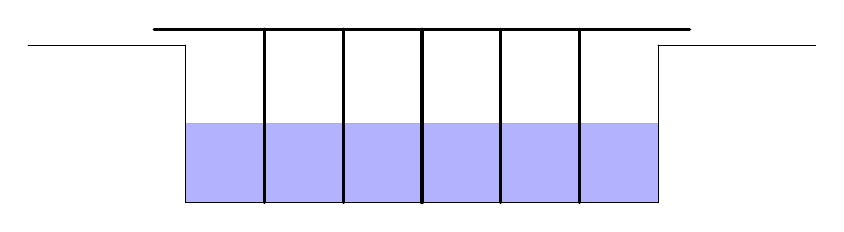
\begin{tikzpicture}[line cap=round,line join=round,>=triangle 45,x=1cm,y=1cm]
            
            \draw [fill=blue,opacity=0.3] (-3,1) rectangle (3,0);
            \draw [] (-5,2)-- (-3,2);
            \draw [] (-3,2)-- (-3,0);
            \draw [] (-3,0)-- (3,0);
            \draw [] (3,0)-- (3,2);
            \draw [] (3,2)-- (5,2);
            \draw [very thick] (-3.4,2.2)-- (3.4,2.2);
            \draw [very thick] (-2,2.2)-- (-2,0);
            \draw [very thick] (-1,0)-- (-1,2.2);
            \draw [very thick] (0,2.2)-- (0,0);
            \draw [very thick] (1,0)-- (1,2.2);
            \draw [very thick] (2,2.2)-- (2,0);
            \end{tikzpicture}
    \end{center}
    where the horizontal platform is known as the \textbf{beam} and the vertical supports are known as \textbf{posts} (which comes from the german word for tree)
    \item Disadvantages of this bridge is that it can easily break and become unusable in the event of a flood. This can be modified to become a \textbf{truss} bridge:
    \begin{center}
        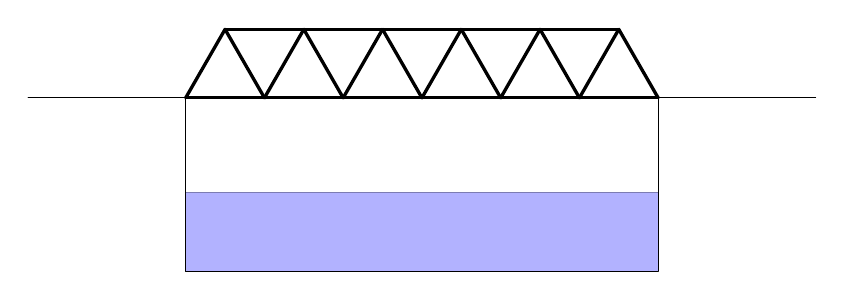
\begin{tikzpicture}[line cap=round,line join=round,>=triangle 45,x=1cm,y=1cm]
            \draw [fill=blue,opacity=0.3] (-3,1) rectangle (3,0);
            \draw [] (-5,2.2)-- (-3,2.2);
            \draw [] (-3,2.2)-- (-3,0);
            \draw [] (-3,0)-- (3,0);
            \draw [] (3,0)-- (3,2.2);
            \draw [] (3,2.2)-- (5,2.2);
            \draw [very thick] (-3,2.2)-- (3,2.2);

            \foreach \x in {-3,-2,...,2}
            \draw [very thick] (\x ,2.2)-- (0.5+\x ,3.07);

            \foreach \x in {-3,-2,...,2}
            \draw [very thick] (\x+1,2.2)-- (0.5+\x ,3.07);

            \draw [very thick] (-2.5,3.07) -- (2.5,3.07);
            \end{tikzpicture}
    \end{center}
    However this type of bridge needs constant maintenance and none of the truss bridges the Romans have built lasted to today.
    \item One of the oldest bridges (est. 5000 BC) was built across a large pond, known as the ``Sweet Track.'' The bridge was built in an X-shape and people could walk on top:
    \begin{center}
        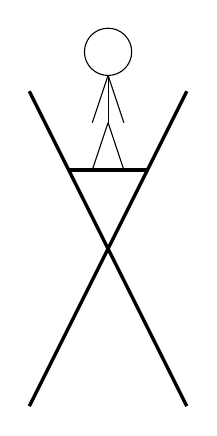
\begin{tikzpicture}
            \draw [very thick] (-1,2)-- (1,-2);
            \draw [very thick] (-1,-2)-- (1,2);
            \draw [] (0,2.2)-- (0,1.6);
            \draw [] (0,2.5) circle (0.3cm);
            \draw [very thick] (-0.5,1)-- (0.5,1);
            \draw [] (0,1.6)-- (-0.2,1);
            \draw [] (0,1.6)-- (0.2,1);
            \draw [] (0,2.2)-- (-0.2,1.6);
            \draw [] (0,2.2)-- (0.2,1.6);
        \end{tikzpicture}
    \end{center}
    \item Another form of bridge is suspended by hanging chains, known as a \textbf{suspension bridge}. A strong \textit{main cable} is pulled over two towers and fixed into concrete supports. Secondary \textit{hanging cables} run vertically and add support to the bridge.
    \begin{center}
        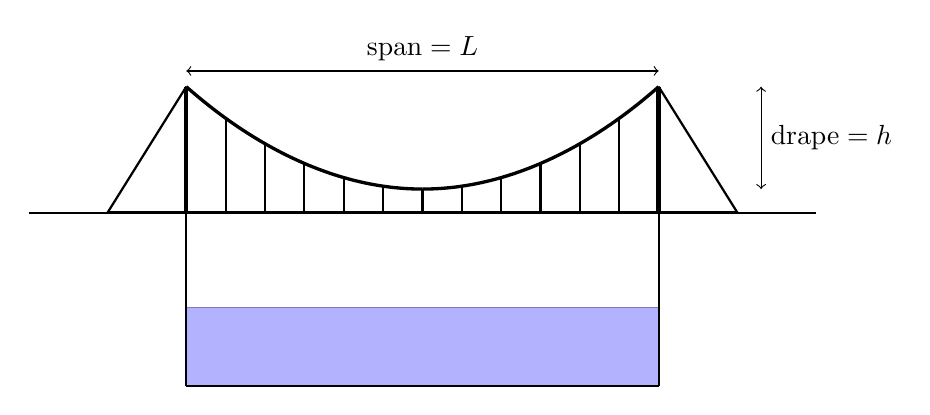
\begin{tikzpicture}
            \draw [fill=blue,opacity=0.3] (-3,1) rectangle (3,0);
            \draw [thick] (-5,2.2)-- (-3,2.2);
            \draw [thick] (-3,2.2)-- (-3,0);
            \draw [thick] (-3,0)-- (3,0);
            \draw [thick] (3,0)-- (3,2.2);
            \draw [thick] (3,2.2)-- (5,2.2);
            
            \draw [very thick] (0,2.5) parabola (3,3.8);
            \draw [very thick] (0,2.5) parabola (-3,3.8);
            \draw [very thick] (-4,2.2)-- (4,2.2);

            \foreach \x in {-2.5,-2,...,2.5}
            \draw [thick] (\x ,2.2)-- (\x ,0.144*\x*\x+2.5);

            \draw [ultra thick] (-3 ,2.2)-- (-3,3.8);
            \draw [thick] (-4,2.2) -- (-3,3.8);
            \draw [ultra thick] (3 ,2.2)-- (3,3.8);
            \draw [thick] (4,2.2) -- (3,3.8);
          
            \draw [<->] (-3,4) -- (3,4) node[midway,above] {$\text{span}=L$};
            \draw [<->] (4.3,2.5) -- (4.3,3.8) node[midway,right] {$\text{drape}=h$};
        \end{tikzpicture}
    \end{center}
    The ratio of the drape to the span is very important in determining how well the bridge is able to support the load. A typical ratio would be $L:h=10:1$.
    \item The \textbf{dead load} refers to the weight of the bridge as is, and the \textbf{live load} refers to the actual cars and people that need to cross the bridge. 
    \item Under its own weight or under a constant force, a piece of rope or flexible material will form the shape of a \textbf{catenary}, which is a shape that minimizes the potential energy of the system.
    \item The \textbf{catenary} shape very closely resembles that of a parabola, at least for small enough values, such that for most purposes it can be approximated as such.
\end{itemize}
\newpage
\section{Crystallographic Planes and Directions}
\begin{itemize}
    \item We develop a set of notation to describe directions. It comes with a set of rules:
    \begin{itemize}
        \item Translate vector, if it simplifies things.
        \item Determine projection onto $x$, $y$, $z$.
        \item Reduce to lowest integers.
        \item Enclose in square brackets (negative signs are moved above, no commas)
    \end{itemize}
    \begin{example}
        We can find the crystallographic directions of both the blue and the red vectors in the figure below.
        \begin{center}
            \incfig{crystallographic_intro}
        \end{center}
        For the blue vector, we first let the tail by the origin. The vector travels $1$ in the negative $x$ direction, $0$ in the $y$ direction, and $-1$ in the negative $z$ direction, which gives $[\bar{1}\,0\,\bar{1}]$.
        \vspace{2mm}

        For the red vector, it travels in the negative $y$ direction for $0.5$ and in the negative $z$ direction for $1$ so we get, after getting rid of fractions: $[0\,\bar{1}\,\bar{2}]$.
    \end{example}
    \item To denote a family of directions, we can use braket notation. All face diagonals can be written as:
    \begin{equation}
        <0\,1\,1>
    \end{equation}
    which includes:
    \begin{equation}
        [0\,1\,1],\, [0\,\bar{1}\,1],\, [0\,1\,\bar{1}],\, [1\,0\,1], \ddots
    \end{equation}
\end{itemize}
\newpage
\section{Cylindrical, Spherical Coordinates, Taylor Series, Jacobian}
\begin{itemize}
    \item In \textbf{cylindrical coordinates}, we can represent a point in $\mathbb{R}^3$ as 
    \begin{equation}
        P(x,y,z) = P(r,\theta,z).
    \end{equation}
    We can describe a region as 
    \begin{equation}
        Q = \{(x,y,z) | (x,y)\in R, u_1(x,y)\le z\le u_2 (x,y)\}
    \end{equation}
    where
    \begin{equation}
        R= \{(r,\theta)|\alpha\le \theta\le \beta, h_1(\theta)\le r\le h_2(\theta)\}
    \end{equation}
    and the integral can be written as 
    \begin{align}
        \iiint\limits_Q f(x,y,z)\dd{V} &=\iint\limits_R \left[\int_{u_1(x,y)}^{u_2(x,y)}\right]\dd{A} \\ 
        &= \int_\alpha^\beta \int_{h_1(\theta)}^{h_2(\theta)}\int_{u_1(r\cos\theta,r\sin\theta)}^{u_2(r\cos\theta,r\sin\theta)}f(r\cos\theta,r\sin\theta,z)r\dd{z}\dd{r}\dd{\theta.} 
    \end{align}
    \item In spherical coordinates, a point can be represented by 
    \begin{equation}
        P(x,y,z)=P(\rho,\theta,\phi)
    \end{equation}
    where $\theta$ is the same as the one in cylindrical coordinates\footnote{This is the common convention in physics. However, many mathematics texts mix up $\theta$ and $\phi$}. We have 
    \begin{align}
        x &= \rho\sin\phi\cos\theta \\ 
        y &= \rho\sin\phi\sin\theta \\ 
        z &= \rho \cos\phi 
    \end{align}
    and 
    \begin{equation}
        \rho^2 = x^2+y^2+z^2.
    \end{equation}
    \item The volume in spherical coordinates is given by 
    \begin{equation}
        \dd{V} = \rho^2 \sin\phi \dd{\rho}\dd{\phi}\dd{\theta}
    \end{equation}
    \begin{idea}
        We can create a change of basis from $\hat{i},\hat{j},\hat{k}$ to $e_\rho$, $e_\theta$, and $e_\phi$ as follows: 
        \begin{align}
            e_\rho &= \sin\phi\cos\theta \hat{i} +\sin\phi\cos\theta\hat{j} +\cos\phi \hat{k} \\ 
            e_\theta &= -\sin\theta \hat{i} + \cos\theta\hat{j} + 0\hat{k} \\ 
            e_\phi &= \cos\phi\cos\theta \hat{i} + \cos\phi\sin\theta \hat{j} - \sin\theta \hat{k} 
        \end{align}
        which can be represented in the following transformation: 
        \begin{equation}
            [v]_\text{cartesian} = \begin{bmatrix}
                \cos\theta\sin\phi & -\sin\theta & \cos\theta\cos\phi \\ 
                \sin\theta\sin\phi & \cos\theta & \sin\theta\cos\phi \\ 
                \cos\phi & 0 & -\sin\phi
            \end{bmatrix}[v]_\text{spherical}
        \end{equation}
        That is, if you coordinates in the spherical basis, then you can use this transformation to get the coordinates in the cartesian basis. This means that at a particular $\theta$ and $\phi$, the unit vector $e_\rho = (1,0,0)$ maps to $(\cos\theta\sin\phi, \sin\theta\sin\phi, \cos\phi),$ which is what we expect. Let this transformation matrix be $M$. Since $M$ is composed of only unit vectors, the inverse is the transpose: 
        \begin{equation}
            [v]_\text{spherical} = \begin{bmatrix}
                \cos\theta\sin\phi & \sin\theta\sin\phi & \cos\phi \\ 
                -\sin\theta & \cos\theta & 0 \\ 
                \cos\theta\cos\phi & \sin\theta\cos\phi & -\sin\phi 
            \end{bmatrix}[v]_\text{cartesian}
        \end{equation}
        So any vector written in the cartesian basis can be written in terms of the spherical basis vectors via this transformation.
    \end{idea}
    \item \textbf{Taylor Series for Two-Variable Functions:} Suppose we are given $f(x_0,y_0)$ and want to approximate $f(x_0+\Delta x,y_0+\Delta y).$ Suppose there projections on the $xy$ plane is $P$ and $Q$. We can parametrize the line segment $PQ$ as 
    \begin{align}
        x(t) = x_0 + t\Delta x \\ 
        y(t) = y_0 + t\Delta y
    \end{align}
    where $0 \le t \le 1$. We can then define 
    \begin{equation}
        F(t) = f(x_0+t\Delta x,y_0+t\Delta y)
    \end{equation}
    which is a one-variable function, which we can approximate using the one dimensional Taylor Series: 
    \begin{equation}
        F'(t) = \frac{\partial f}{\partial x}\Delta x + \frac{\partial f}{\partial y}\Delta y
    \end{equation}
    The second derivative is 
    \begin{equation}
        F''(t)  = \frac{\partial^2 f}{\partial x^2}\Delta x^2 + 2\frac{\partial^2 f}{\partial x\partial y}\Delta x\Delta y + \frac{\partial^2 f}{\partial y^2}\Delta y^2
    \end{equation}
    The third derivative is
    \begin{equation}
        F'''(t) = \frac{\partial^3f}{\partial x^3}\Delta x^3 + 3\frac{\partial^3 f}{\partial x^2\partial y}\Delta x^2\Delta y + 3\frac{\partial^3 f}{\partial x\partial y^2}\Delta x\Delta y^2 + \frac{\partial^3f}{\partial y^3}\Delta y^3 .
    \end{equation}
    Therefore: 
    \begin{equation}
        F(t_0+\Delta t)\approx F(t_0) + F'(t_0)\Delta t + \frac{1}{2!}F''(t_0)\Delta t^2 + \cdots + \frac{F^{(n)}(t_0)\Delta t}{n!}
    \end{equation}
    % \item Alternatively, we can write 
    % \begin{equation}
    %     f(x_0,y_0) \approx f(x_0,y_0) + \frac{\partial f}{\partial x}\Bigg|_{(x_0,y_0)}(x-x_0) + \frac{\partial f}{\partial y}\Bigg|_{(x_0,y_0)}(y-y_0) + \frac{1}{2!}\left(\frac{\partial^2 f}{\partial x}\Bigg|_{(x_0,y_0)}(x-x_0)^2\right)
    % \end{equation}
    \item \textbf{Change of Variables in Multiple Integrals:} Consider a bijective mapping between a region $S$ in the $uv$ plane to a region $R$ in the $xy$ plane. We can partition both regions into $N$ regions.
    
    Specifically, let us partition $S$ into square regions. Consider an arbitrary region with vertices $\bar{A}(u_0,v_0)$, $\bar{B}(u_0+\Delta u, v_0)$, $\bar{C}(u_0,v_0+\Delta v)$, and $\bar{D}$. Let the subregion be denoted as $S_i$ with area $\Delta A_S$.

    Suppose we have the mapping 
    \begin{align}
        x &= g(u,v) \\ 
        y &= h(u,v)
    \end{align}
    such that $\bar{X}\mapsto X$. If $\Delta u$ and $\Delta v$ are sufficiently small, then $R_i=ABCD$ is a parallelogram. Therefore: 
    \begin{equation}
        \Delta A_R \approx \text{area of the parallelogram} = \lVert \vec{AB} \times \vec{AC}\rVert.
    \end{equation} 
    Note that $\vec{AB}=\Delta x_1 \hat{i}+\Delta y_1 \hat{j}$ and $\vec{AC} = \Delta x_2\hat{i}+\Delta y_2 \hat{j},$ so their cross product is 
    \begin{equation}
        \lVert \vec{AB}\times \vec{AC} \rVert = |\Delta x_1\Delta y_2 - \Delta x_2\Delta y_1| 
    \end{equation}
    From our linear approximation, we can write 
    \begin{align}
        \Delta x_1 &\approx g_u(u_0,v_0)\Delta u \\ 
        \Delta x_2 &\approx g_v(u_0,v_0)\Delta v \\ 
        \Delta y_1 &\approx h_u(u_0,v_0)\Delta u \\ 
        \Delta y_2 &\approx h_v(u_0,v_0)\Delta v
    \end{align}
    To sum it up, we have 
    \begin{equation}
        \Delta A_R = \left|\det \begin{bmatrix}
            g_u(u_0,v_0) & g_v(u_0,v_0) \\ 
            h_u(u_0,v_0) & h_v(u_0,v_0)
        \end{bmatrix}\right| \Delta u\Delta v
    \end{equation}
    \begin{definition}
        The determinant of the derivative matrix is called the Jacobian ($J$) of the transformation. 
        \begin{equation}
            J = \det \begin{bmatrix}
                g_u & g_v \\ 
                h_u & h_v
            \end{bmatrix} = \det\begin{bmatrix}
                x_u & x_v \\ 
                y_u & y_v
            \end{bmatrix} \equiv \frac{\partial(x,y)}{\partial(u,v)}
        \end{equation}
        given 
        \begin{align}
            x &= g(u,v) \\ 
            y &= h(u,v)
        \end{align}
        Therefore, 
        \begin{equation}
            \Delta A_R \approx |J|\Delta A_S
        \end{equation}
    \end{definition}
    \begin{theorem}
        Assuming that 
        \begin{itemize}
            \item $f$ is continuous
            \item $g$ and $h$ are functions that have continuous first derivatives
            \item The transformation is $1-1$.
            \item The Jacobian $J$ is nonzero
        \end{itemize}
        we can write 
        \begin{equation}
            \iint\limits_R f(x,y)\dd{A} = \iint_S f(g(u,v),h(u,v))\left|\frac{\partial(x,y)}{\partial(u,v)}\right|\dd{u}\dd{v}.
        \end{equation}
        Note the similarity between this and the single variable case 
        \begin{equation}
            \int_a^b f(x) \dd{x} = \int_c^d f(x(u)) \frac{\dd{x}}{\dd{u}} \dd{u}
        \end{equation}
    \end{theorem}
    \begin{example}
        Suppose we wish to evaluate the integral $\iint\limits_R (x^2+2xy)\dd{A}$ where $R$ is the region bounded by the lines 
        \begin{align}
            y &= 2x+3 \\ 
            y &= 2x+1 \\ 
            y &= 5-x \\ 
            y &= 2-x
        \end{align}
        Notice that this is a rotated rectangle, so let's try to switch this into a non-rotated rectangle with the bounds: 
        \begin{align}
            u &= 3 \\ 
            u &= 1 \\ 
            v &= 5 \\ 
            v &= 2
        \end{align}
        by the transformation 
        \begin{align}
            x &= \frac{1}{3}(v-u) \\ 
            y &= \frac{1}{3}(2v+u).
        \end{align}
        The Jacobian is 
        \begin{equation}
            J = \det \begin{bmatrix}
                \frac{\partial x}{\partial u} & \frac{\partial x}{\partial v} \\ 
                \frac{\partial y}{\partial u} & \frac{\partial y}{\partial v}
            \end{bmatrix} = \det\begin{bmatrix}
                -1/3 & 1/3 \\ 
                1/3 & 2/3
            \end{bmatrix} = -\frac{1}{3}
        \end{equation}
        which gives 
        \begin{equation}
            \iint\limits_R (x^2+2xy)\dd{A} = \iint_S \left[\frac{1}{3}(v-u)^2+\frac{2}{3}(v-u)(2v+u)\right]|J| \dd{u}\dd{v}
        \end{equation}
        where $S=\{(u,v)| 1 \le u \le 3, 2 \le v\le 5\}$
    \end{example}
    \item For triple integrals, the Jacobian is 
    \begin{equation}
        \frac{\partial (x,y,z)}{\partial (u,v,w)} = \det \begin{bmatrix}
            \frac{\partial x}{\partial u} & \frac{\partial x}{\partial v} & \frac{\partial x}{\partial w} \\ 
            \frac{\partial y}{\partial u} & \frac{\partial y}{\partial v} & \frac{\partial y}{\partial w} \\ 
            \frac{\partial z}{\partial u} & \frac{\partial z}{\partial v} & \frac{\partial z}{\partial w}
        \end{bmatrix}
    \end{equation}
    \item \textbf{Successive Transformations:} Suppose we have $x=x(u,v), y=y(u,v)$ and $u=u(s,t)$ and $v=v(s,t).$ Then
    \begin{equation}
        \frac{\partial(x,y)}{\partial(s,t)} = \frac{\partial(x,y)}{\partial(u,v)}\cdot \frac{\partial (u,v)}{\partial (s,t)}
    \end{equation}
    \item \textbf{Back Transformations:} Recall that when we transform a region $R$ to a region $S$ with some transformation $T$, then 
    \begin{equation}
        \dd{A}_R = \left|\frac{\partial (x,y)}{\partial (u,v)}\right|\dd{A}_S
    \end{equation}
    and 
    \begin{equation}
        \dd{A}_S = \left|\frac{\partial (u,v)}{\partial (x,y)}\right|\dd{A}_R
    \end{equation}
    \begin{theorem}
        Jacobians satisfy the property: 
        \begin{equation}
            \frac{\partial(x,y)}{\partial(u,v)} = \left(\frac{\partial(u,v)}{\partial (x,y)}\right)^{-1}
        \end{equation}
        or 
        \begin{equation}
            J_{S\rightarrow R} = \frac{1}{J_{R\rightarrow S}}
        \end{equation}
    \end{theorem}
    \begin{idea}
        This is important since if we know $u=f(x,y)$ and $v=g(x,y)$, then we can calculate the Jacobian without finding the inverse. 
    \end{idea}
\end{itemize}
\newpage
\section{Line Integrals, Fundamental Theorem, Green's Theorem, and Parametric Surfaces}
\begin{itemize}
    \item Suppose we have a line in $\mathbb{R}^3$ and we wish to evaluate a function along this line.
    \item We can break this line into segments $\Delta s_i$ and sum up 
    \begin{equation}
        f(x_i^*,y_i^*)\Delta s_i
    \end{equation}
    Taking the limit, we get
    \begin{equation}
        \int\limits_C f(x,y) \dd{s}
    \end{equation}
    \item Taking $f(x,y)=1$ gives the length of the line segment $C$. 
    \item We need to assume that
    \begin{itemize}
        \item $f$ is continuous
        \item $C$ is smooth ($\vec{r}(t)$ is continuous and $\vec{r}'(t) \neq 0$ except at endpoints)
    \end{itemize}
    and have the curve be parametrized 
    \begin{equation}
        \vec{r}(t) = x(t)\hat{i}+y(t)\hat{j}
    \end{equation}
    so we can write 
    \begin{equation}
        \dd{s} = \sqrt{x'(t)^2 + y'(t)^2}\dd{t}.
    \end{equation}
    \begin{example}
        Suppose we wish to find the center of mass of a semi-circular length of wire. The length density is to be taken as constant. Note that $\bar{x}=0$ by symmetry. The moment about the $x$ axis is then: 
        \begin{equation}
            m\bar{y} = \int\limits_C y\rho \dd{s}.
        \end{equation}
        We can parametrize $\vec{r}(t) = a\cos t \hat{i} + a\sin t\hat{j}$ and $\dd{s} = a\dd{t}.$ Therefore: 
        \begin{equation}
            \bar{y} = \frac{1}{m}\int\limits_C y\rho \dd{s} = \frac{1}{m}\int_0^\pi a\sin t\rho a \dd{t} = \frac{2a}{\pi}.
        \end{equation}
    \end{example}
    \item In the special case where $C$ is parallel to the $x$ axis, then we can reduce it to the familiar single-variable integral.
    \item \textbf{Three-Dimensions:} We can easily extend it to three dimensions: 
    \begin{equation}
        \int_C f(x,y,z) \dd{s} = \int_a^b f(\vec{r}(t)) \cdot \lVert \vec{r}'(t)\rVert \dd{t} 
    \end{equation}
    \item For a piecewise smooth curve, we need to break up the line integral into several smaller ones.
    \begin{idea}
        Let $f(x,y)$ be a scalar. Then $\int_C f(x,y) \dd{s} = \int_{-C}f(x,y) \dd{s}$. This is because $\dd{s}$ is always positive.
    \end{idea}
    \item Suppose we have a vector field 
    \begin{equation}
        \vec{F}(x,y,z) = P(x,y,z)\hat{i} + Q(x,y,z)\hat{j} + R(x,y,z)\hat{k} = \vec{F}(\vec{r})
    \end{equation}
    \item The work done along a curve $C$ is given by 
    \begin{equation}
        \int\limits_C \vec{F}(x,y,z)\cdot \vec{T}(x,y,z)\dd{s} = \int_a^b \vec{F}(\vec{r}(t)) \cdot \vec{r}'(t) \dd{t} = \int\limits_C \vec{F}\cdot \vec{r}
    \end{equation}
    \item NOte that if we have $\vec{r}(t)=x(t)\hat{i}+y(t)\hat{j} + z(t)\hat{k}$ where $a\le t\le b$, then 
    \begin{equation}
        \frac{d\vec{r}(t)}{dt} = \frac{dx}{dt}\hat{i} + \frac{dy}{dt}\hat{j} + \frac{dz}{dt} \hat{k}
    \end{equation}
    so 
    \begin{align}
        \int\limits_C \vec{F}\cdot \dd{\vec{r}} &= \vec{F}(\vec{r}(t))\cdot \vec{r}'(t) \dd{t} \\ 
        &= \int_a^b (P\hat{i}+Q\hat{j}+R\hat{k})\cdot \left(\frac{dx}{dt}\hat{i} + \frac{dy}{dt}\hat{j} + \frac{dz}{dt}\hat{k}\right)\dd{t} \\ 
        &= \int\limits_C P \dd{x} + \int\limits_C Q \dd{y} + \int\limits_C R \dd{z}
    \end{align}
    \begin{definition}
        A vector field $\vec{F}$ is called a conservative vector field if it is the gradient of some scalar function $\vec{\nabla} f.$ In this situation, the scalar function is called a potential function of $\vec{F}$.
    \end{definition}
    \item Suppose that $\vec{F}(x,y,z)=\vec{\nabla}f(x,y,z)$ and let $C$ be a smooth curve given by $\vec{r}(t) = x(t)\hat{i} + y(t)\hat{j} + z(t)\hat{k}$ where $a\le t\le b.$ Then 
    \begin{align}
        \vec{\nabla}f(\vec{r(t)})\cdot \vec{r}'(t) &= \left(\frac{\partial f}{\partial x}\hat{i} + \frac{\partial f}{\partial y}\hat{j} + \frac{\partial f}{\partial z}\hat{k}\right)\cdot \left(\frac{dx}{dt}\hat{i} + \frac{dy}{dt}\hat{j} + \frac{dz}{dt}\hat{k}\right) \\ 
        &= \frac{\partial f}{\partial x}\frac{dx}{dt} + \frac{\partial f}{\partial y}\frac{dy}{dt} + \frac{\partial f}{\partial z}\frac{dz}{dt} \\ 
        &= \frac{df}{dt}.
    \end{align}
    Therefore, the line integral becomes 
    \begin{equation}
        \int_a^b \vec{\nabla}f(\vec{r}(t))\cdot \vec{r}'(t) \dd{t} = \int_a^b \frac{d}{dt} (f(\vec{r}(t)))\dd{t} = f(\vec{r}(b))-f(\vec{r}(a))
    \end{equation}
    \begin{theorem}
        The \textbf{fundamental theorem of line integrals} tells us that
        \begin{equation}
            \int\limits_C \vec{\nabla}f\cdot \dd{\vec{r}} = f(\vec{r}(b))-f(\vec{r}(a))
        \end{equation}
    \end{theorem}
    \item The reverse is also true. If $\oint\limits_C \vec{F} \cdot \dd{r} = 0$ for every piecewise smooth closed curve $C$ over a domain $D$, then $\int\limits_{C_1}\vec{F}\cdot \dd{\vec{r}}$ is path independent for any piecewise smooth path $C_1$ in $D$: 
    \begin{equation}
        \oint\limits_C \vec{F} \cdot \dd{\vec{r}} = 0 \implies \int\limits_{C_1}\vec{F}\cdot{\vec{r}} + \int\limits_{C_2}\vec{F}\cdot \dd{\vec{r}} = 0
    \end{equation}
    where 
    $C=C_1\cup C_2$.
    \begin{theorem}
        Given a vector field $\vec{F}$, if $\int\limits_C \vec{F}\cdot \dd{\vec{r}}$ is path independent for every piecewise smooth curve $C$ in the domain of $\vec{F}$, then $\vec{F}$ is a conservative vector field and therefore there exists a scalar function $f$ such that $\vec{\nabla}f=\vec{F}$.
    \end{theorem}
    \item If one of the following is true, then the other two are also true: 
    \begin{itemize}
        \item $\vec{F}$ is conservative ($\vec{F}=\vec{\nabla}F$)
        \item $\oint\limits_C \vec{F}\cdot \dd{\vec{r}} = 0$ for every piecewise smooth closed curve.
        \item $\int\limits_C \vec{F}\cdot \dd{\vec{r}}$ is path independent for all piecewise smooth $C$ between any two fixed points.
    \end{itemize}
    \item Suppose we have $\vec{F}(x,y)=P(x,y)\hat{i} + Q(x,y)\hat{j}.$ We know $\vec{F}$ is conservative if and only if 
    \begin{align}
        \vec{F} &= \vec{\nabla}f \\ 
        P\hat{i}+Q\hat{j} &= \frac{\partial f}{\partial x}\hat{i} + \frac{\partial f}{\partial y}\hat{j}
    \end{align}
    This gives $P=\frac{\partial f}{\partial x}$ and $Q =\frac{\partial f}{\partial y}$. Note that \begin{equation}
        \frac{\partial P}{\partial y}=\frac{\partial ^2 f}{\partial y\partial x}=\frac{\partial^2 f}{\partial x\partial y}=\frac{\partial Q}{\partial x.}
    \end{equation}
    This leads to our next theorem: 
    \begin{theorem}
        If $\frac{\partial P}{\partial y}=\frac{\partial Q}{\partial x},$ then $\vec{F}=\vec{\nabla} f$.
    \end{theorem}
    \item We introduce some terminology to prelude \textbf{Green's Theorem}
    \begin{definition}
        A simple curve is a curve that does not intersect itself, except at its endpoints. 
    \end{definition}
    \begin{definition}
        A curve has positive orientation if it traverses counterclockwise, and negative if you traverse it clockwise.
    \end{definition}
    \begin{definition}
        Let $C$ be a positively oriented, piecewise-smooth simple closed curve in the plane and let $R$ be the region bounded by $C$. IF $P(x,y)$ and $Q(x,y)$ are continuous and have continuous first partial derivatives throughout the region $R$, then 
        \begin{equation}
            \oint\limits_C P(x,y)\dd{x} + Q(x,y)\dd{y} = \iint\limits_R \left(\frac{\partial Q}{\partial x} - \frac{\partial P}{\partial y}\right) \dd{x}\dd{y}
        \end{equation}
    \end{definition}
    \begin{example}
        Let's verify Green's Theorem for the integral $\oint\limits_C y\dd{x}-x\dd{y}$ where $C$ is the curve $C:x^2+y^2+1$ traversed counterclockwise.
        \vspace{2mm}

        \textit{Method 1:} Let us first check if $\vec{F}=y\hat{i}-x\hat{j}$ is conservative. However, $P_y=1$ and $Q_x=-1$ so it is not conservative.
        \vspace{2mm}
        
        \textit{Method 2:} We have $\vec{r}(t)=\cos t\hat{i}+\sin t\hat{j}$ and 
        \begin{equation}
            \oint \vec{F}\cdot \dd{\vec{r}} = \int_{t=0}^{2\pi}\vec{F}(\vec{r}(t)) \cdot \vec{r}'(t) \dd{t} = \int_0^{2\pi} (\sin t\hat{i}-\cos t\hat{j})\cdot (-\sin t\hat{i}+\cos t\hat{j}) \dd{t} = -2\pi 
        \end{equation}
        \vspace{2mm}

        \textit{Method 3:} Using Green's Theorem, we have 
        \begin{equation}
            \oint\limits_C P\dd{x} + Q\dd{y} = \iint\limits_R (Q_x-P_y)\dd{A} = \iint\limits_R (-1-1) \dd{A} = -2\iint\limits_R\dd{A} = -2(\pi \cdot 1^2)
        \end{equation}
    \end{example}
    \begin{warning}
        Green's Theorem is only true for curves with positive orientations. If the curve has a negative orientation, then we need to include a factor of $-1$.
    \end{warning}
    \item Curves can be parametrized by a single parameter. Similarly, surfaces can be parametrized by two parameters: 
    \begin{equation}
        \vec{r}(u,v) = x(u,v)\hat{i} + y(u,v)\hat{j} + z(u,v)\hat{k}
    \end{equation}
    \item The easiest way to parametrize a surface $S:z=f(x,y)$ is to let $x=u,y=v,z=f(u,v)$ to get 
    \begin{equation}
        \vec{r}(u,v)=u\hat{i}+v\hat{j}+f(u,v)\hat{k}
    \end{equation}
    \begin{example}
        We can parametrize an upper hemisphere given by the equation $x^2+y^2+z^2=a^2$. We get 
        \begin{equation}
            \vec{r}(u,v) = u\hat{i}+v\hat{j} + \sqrt{a^2-u^2-v^2}\hat{k}
        \end{equation}
        Similarly in spherical coordinates, we can parametrize it as $\rho= a$, $0\le \theta \le 2\pi$, and $0\le \phi \le \pi/2$.
    \end{example}
    \item \textbf{Tangent Planes:} Let $S$ be a surface parametrized by the differentiable vector function $\vec{r}=\vec{r}(u,v)=x(u,v)\hat{i}+y(u,v)\hat{j} + z(u,v)\hat{k}$ where $(u,v) \in D.$ Then: 
    \begin{align}
        \vec{r}_v(u_0,v_0) &= \frac{\partial \vec{r}(u,v)}{\partial v}\bigg|_{(u_0,v_0)} \\ 
        \vec{r}_u(u_0,v_0) &= \frac{\partial \vec{r}(u,v)}{\partial u}\bigg|_{(u_0,v_0)}
    \end{align}
    are the tangent vector to $C_1 = \vec{r}(u_0,v)$ and $C_2=\vec{r}(u,v_0)$, respectively.
    \begin{definition}
        For every point on a surface $S$, if $\vec{r}_u\times \vec{r}_v \neq \vec{0}$, then such a surface is called a smooth surface. Then $\vec{r}_u(u_0,v_0)\times \vec{r}_v(u_0,v_0)$ is perpendicular to the surface at point $P$.
    \end{definition}
    \begin{theorem}
        The surface area is given by 
        \begin{equation}
            S = \iint\limits_D \lVert \vec{r}_u \times \vec{r}_v \rVert \dd{u}\dd{v}
        \end{equation}
    \end{theorem}
\end{itemize}
\newpage
\section{Integration}
\begin{itemize}
    \item Let $R=\prod_{i=1}^n [a_i,b_i]$ be a rectangle in $\mathbb{R}^n$ and let $f:\mathbb{R}\rightarrow \mathbb{R}$ be a bounded function.
    \item A partition $\mathcal{P}$ of $R$ is a sequence $(P_i)^n$ where each $P_i$ is a partition of $[a_i,b_i]$, i.e. $P:a_i = t_{i0} < t_{i1} < t_{i2} < \cdots \le t_{iN_i}=b_i.$
    \item A subrectangle $S$ relative to a partition $\mathcal{P}$, you choose integers $1 \le j_i \le N_i$ for $i=1,\dots, n$ with $j=(j_1\, \cdots\, j_n)$, we have 
    \begin{equation}
        S_j = \prod_{i=1}^n [t_{i,j_{i-1}}, t_{ij_i}] \ni x
    \end{equation}
    (note: could be wrong)
    \item Notation: We say $S \in P$
    \item If $S \neq S' \in P$ then $S$ intersects $S'$ at most on boundaries.
    \item $\bigcup_{S\in P}S = R$.
    \item $\left|\{S:S\in P\}\right|=\prod N_i$
    \begin{definition}
        The volume of $R$ is given by
        \begin{equation}
            V(R) = |R| = \prod (b_i-a_i)
        \end{equation}
    \end{definition}
    \begin{proposition}
        If $P$ is a partition of $R$,
        \begin{equation}
            \sum_{S\in P}V(S) = V(R)
        \end{equation}
    \end{proposition}
    \item Normally,
    \begin{equation}
        \sum \prod_{i=1}^n (t_{ij_i}-t_{i,j_{i-1}})
    \end{equation}
\end{itemize}
\newpage
\section{Lecture 8}
\begin{itemize}
    \item A ``continuous function'' is intuitively clear, but how do we define it rigorously?
    \begin{definition}
        $f(x)$ is ``continuous at $c$'' if
        \begin{equation}
            \lim_{x\to c}f(x)=f(c)
            \label{eq:}
        \end{equation}
    \end{definition}
    \begin{definition}
        A function $f(x)$ is discontinuous at $c$ if it is not continuous.
    \end{definition}
    \item There are various types of discontinuity:
    \begin{itemize}
        \item \textbf{Jump Discontinuity-} For example:
        \begin{equation}
            f(x)=\frac{|x|}{x}
            \label{eq:}
        \end{equation}
        \item \textbf{Removable Discontinuity-} For example:
        \item Discontinuity because either $f(c)$ DNE or $\displaystyle \lim_{x\to c} f(x)$ DNE, or both.
    \end{itemize}
    \item There are also continuity theorems.
    \begin{theorem}
        If $f(x)$ is continuous at every $x\in[a,b]$, then $f(x)$ is integrable on $[a,b]$ i.e. $\int_a^b f(x) \dd{x}$ exists.
    \end{theorem}
    \begin{theorem}
        Given $f$, $g$ is continuous at $a$, then $f(x)+g(x)$ is continuous at $a$.
    \end{theorem}
    \begin{prooof}
        Apply the additivity L.T lmao.
    \end{prooof}
    \item There is also such a thing as a one-sided continuity.
    \begin{definition}
        $f(x)$ is continuous on the right at $c$ if $\displaystyle\lim_{x\to c^+}f(x)=f(c)$.
    \end{definition}
    \item amd for an interval.
    \begin{definition}
        $f(x)$ is continuous on $(a,b)$ iff $f(x)$ is continuous at all $x \in (a,b)$.
    \end{definition}
    \begin{definition}
        $f(x)$ is continuous on $[a,b]$ iff $f(x)$ is continuous on $(a,b)$ and $f(x)$ is continuous from the right of $a$ and from the left of $b$.
    \end{definition}
    \begin{theorem}
        If $g(x)$ is continuous at $a$ and $f(x)$ is continuous at $g(a)$, then $f(g(x))$ is continuous at $a$.
    \end{theorem}
    \item We can now introduce the \textbf{Intermediate Value Theorem}. Recap: We simply want there to be a number $q$ such that $q\cdot q=2$, i.e. $\sqrt{2}$ exists. We proved such a number does not exist among the rationals. So we imposed a new axiom CORA and then defined:
    \begin{equation}
        \sqrt{2}=\text{lub}\{x:x^2<2\}
        \label{eq:}
    \end{equation}
    which CORA guarantees exists as a real number. This however doesn't tell us that $\sqrt{2}\cdot\sqrt{2}=2$, but we want to use this result. How can we rigorously prove that:
    \begin{equation}
        [\text{lub}\{x:x^2<2\}]\cdot [\text{lub}\{x:x^2<2\}] = 2
        \label{eq:}
    \end{equation}
    \begin{theorem}
        \begin{enumerate}
            \item Given that $f(x)$ is continuous on $[a,b]$
            \item $C$ is some number such that $f(a)<G(a)<f(b)$.
            \item There exists some $C$ in $[a,b]$ such that $f(C)=G$.
        \end{enumerate}
    \end{theorem}
    \item The point of the IVT is that continuous functions don't skip over any $y$ values. Note that this is a property that intuitively we want continuous functions to have.
    \begin{example}
        Prove that there is a number $c$ such that $c\cdot c=2$ using IVT rather than CORA directly.
        \vspace{2mm}

        Consider $f(x)=x^2$ on $[1,2]$. It is easy to show that $f(x)$ is continuous on $[1,2]$ per the polynomial continuous theorem. Here $f(1)=1$ and $f(2)=4$. Note that $1<2<4$ so $f(1)<2<f(2)$.
        \vspace{2mm}
        
        The IVT shows that there must be some number $c$ where $1<c<2$ in this interval such that $f(c)=c\cdot c=2$. 
    \end{example}
    Note that if reals consisted of rationals only, then the IVT would not be true!
    \item Logically we could have started with the IVA (Intermediate Value Axiom) and used it to prove CORT (Completeness of Reals Theorem). But this would be messy: we would need to define functions before we had finished defining numbers.
    \begin{example}
        Prove there's at least one root of $x^{17}+1=3x$ in $[0,1]$.
        \vspace{2mm}

        Define $f(x)=x^{17}+1-3x$. $f(x)$ is continuous by polynomial continuity theorem. $f(0)=1$ and $f(1)=-1$, so $f(0)>0>f(1)$. By IVT there is some $c$ in $(0,1)$ such that $f(c)=0$. Therefore $c$ is a root of this equation.
    \end{example}
\end{itemize}
\newpage
\section{Model of the Atom}
\begin{itemize}
    \item Light can have a wavelength that ranges from $10^{-11}\si{\meter}$ to $10^3\si{\meter}.$ We can list some common ranges below, listed from shortest wavelength to highest wavelength:
    \begin{itemize}
        \item Gamma Rays
        \item X-Ray
        \item Ultraviolet
        \item Visible (400-700 nm)
        \item Infrared
        \item Microwave
        \item Radio wave
    \end{itemize}
    \item The energy is related to the wavelength via:
    \begin{equation}
        E = \frac{hc}{\lambda}
    \end{equation}
    where $h$ is Planck's constant and $c$ is the speed of light. Oftentimes, we use the electron-volt (eV) unit to characterize energy where:
    \begin{equation}
        1\text{ eV} = 1.602 \times 10^{-19}\si{\joule}
    \end{equation}
    \item In the Bohr-ing model of the atom, it is consisted of a nucleus (with protons + neutrons) and electrons. This model states the following:
    \begin{itemize}
        \item The orbitals are well defined and correspond to a specific energy. Therefore, energy is quantized.
        \item Electrons are able to absorb a specific amount of energy to move into a higher energy state.
    \end{itemize}
    \item In the quantum-mechanical model of the atom, which describes electron orbitals using quantum numbers.
    \begin{itemize}
        \item The principal quantum number $n=1,2,3,4,\dots$ describe the orbital shell. This corresponds to the Bohr model.
        \item The angular momentum quantum number $\ell = 0,1,2,\dots, (n-1)$ or $s,p,d,f$ and they describe the shape of the electron orbital.
        \item The magnetic quantum number, which ranges from $-\ell \le m_\ell \le \ell$. They describe the orientation of the orbitals.
        \item Spin quantum number: $m_s = \pm \frac{1}{2}$.
    \end{itemize}
    \item Subshells are described by the principal and angular momentum quantum numbers and have a very specific energy. Electrons fill these subshells from lowest to highest energy. It is ordered by:
    \begin{equation}
        1s \to 2s \to 2p \to 3s \to 3p \to 4s \to 3d \to 4p \to 5s \to \cdots
    \end{equation}
    For example, carbon has $Z=6$ protons and its electronic configuration is $1s^22s^22p^2$.
    \item For iron with $Z=26$, we may be tempted to write the electronic configuration as:
    \begin{equation}
        1s^22s^22p^63s^23p^64s^23d^6
    \end{equation}
    However, the electronic configuration (due to quantum reasons) that has a lower energy is actually:
    \begin{equation}
        1s^22s^22p^63s^23p^63d^64s^2
    \end{equation}
    Since the last two electrons in the $4s$ orbital is what will be taken away during ionization.
    \begin{idea}
        In this course, we will write electron configurations in increasing principal numbers.
    \end{idea}
    \item Noble (inert) gases don't react easily. A general rule is that octets are stable, and this rule is sometimes written as:
    \begin{equation}
        ns^2np^6
    \end{equation}
    as many atoms want to achieve this configuration.
    \item Covalent, ionic, and metallic bonds exist {\tiny{(sorry if this isn't high school review, i would write more but I still have 8 questions left and it's almost the deadline)}}
    \item Ionization and crystallization energy exist. Salt forms a crystal. Electron affinity also exists. Planning on revisiting this part later so if you're that lone visitor google analytics told me about, please remind me.
    \item In the \textbf{Band Theory}, it attempts to model electrons in a bond. One may naively say that the two electrons share the same state (i.e. same energy, orientation, etc.), but the Pauli exclusion principle forbids that. As a result, they separate out a tiny bit. If we have a large sample, they seem to form a band with a range of possible energies.
    \item Alternatively, if we plot the energy against the intermolecular spacing, we notice that the range of energies separate out if we move from $r=\infty$ to the equilibrium radius $r=r_0$. If we plot it out for the energy of multiple subshells, we'll notice that sometimes there are certain energies in between the bands that no electron can have. This is known as a \textbf{band gap.}
    \begin{idea}
        Bonding creates three bands: The valence band, the band gap, and the conduction band, listed from lowest to highest energy. If the band gap is higher than $4\text{ eV}$, then it is an insulator and if it is less, than it is called a semi-conductor.
    \end{idea}
    \item The important distinction is that for a single atom, the energy of each electron is quantized but if bonding occurs, the energy no longer needs to be quantized.
    \begin{idea}
        We can explain conduction using this model by promoting electrons from the valence band to the conduction band. This reminds us of the ``continuous sea of electron'' analogy for metallic bonding. If there is a band gap, then it becomes a ``Bohr-model'' analogy with electrons jumping up and down between discrete states.
    \end{idea}
    \begin{case}
        The electron configuration of silicon is:
        \begin{equation}
            1s^22s^22p^63s^23p^2
        \end{equation}
        The problem arises is that we know from experiments that silicon has four identical bonds. However, we have 4 electrons at two different energy levels. This shows a limitation in our model and introduces $sp3$ hybridization.
    \end{case}
    \item $sp3$ hybridization is caused by merging the $s$ and $p$ orbitals during bonding, such that the one $s$ orbital and the three $p$ orbitals form into four identical $sp^3$ orbitals. These are known as hybridized orbitals.
    \item It is important to control the electrical conductivity of semiconductors. This is possible by introducing impurities into semiconductors to change their electrical conductivity. The general idea is to delocalize electrons such that they can conduct electricity. In the band theory, it results in a ``hole.'' Although the hole is neutral, since it is surrounded by negative electrons, it can be seen as positive.
    \item This hole is unstable, and as a result electrons will fill it in, creating a new hole from where that electron came from. How quickly electrons can fill this hole characterizes the material's conductivity.
    \item The conductivity $\sigma$ is given by:
    \begin{equation}
        \sigma = nq\mu+n
    \end{equation}
    where $n$ is the number of electrons, $q$ is the fundamental charge, $\mu_n$ is the electron mobility, $p$ is the number of holes, and $\mu_p$ is the hole mobility. For $n=p$, we have:
    \begin{equation}
        \sigma = nq(\mu_n+\mu_p)
    \end{equation}
    \item The conductivity follows the Boltzmann distribution (the textbook said it was the Arrhenius dependence, but that's just chemists trying to steal something physicists came up with):
    \begin{equation}
        \sigma = e^{-E_g/(2kT)}
    \end{equation}
    where $E_g$ is the band gap.
    \item So far, this discussion has revolved around \textit{intrinsic} semi-conductors, which are un-doped. They are not very practical as they are very temperature dependant. If we dope them, the electric properties of the dopant has a large effect on the overall behaviour, and the semi-conductor becomes \textit{extrinsic}.
    \item Extrinsic $n$ type semiconductors are created by adding in free electrons in it. For example, we can add in a \textit{pentravalent} atom (i.e. point defect), which has four electrons that bond with neighbouring carbon electrons, but it has an \textit{extra} free electron. The conductivity is given by:
    \begin{equation}
        \sigma = nq\mu_n
    \end{equation}
    Note that in the background, there is still effects from the instrinsic effects, though they are typically much smaller.
    \item Instead of adding electrons, we can add extra holes in $p$-type extrinsic semiconductors. This is done in a similar way, by adding trivalent impurities such as Boron. The conductivity is then:
    \begin{equation}
        \sigma = pq\mu_p
    \end{equation}
\end{itemize}
\newpage
\section{Thermodynamics}
\begin{itemize}
    \item The laws of physics are time symmetric, meaning on \textit{microscopic} scales, it is impossible to tell the difference between an event happening forwards and happening in reverse. However, on a \textit{macroscopic} scale, an ``arrow of time'' exists.
    \begin{definition}
        A reaction that proceeds without continued input of energy is spontaneous.
    \end{definition}
    \item This definition may create the misconception that exothermic reactions are spontaneous. This is not true, since there is an initial activation energy that is needed to kickstart the reaction, even though it gives off \textit{net} heat. \textit{One reason} is because reactions have multiple steps. Suppose we take the reaction:
    
    \begin{equation}
        \ch{Na_{(s)} + 1/2 Cl_2_{(g)} -> NaCl_{(s)}}
    \end{equation}
    which consists of the following steps:
    \begin{align}
        \ch{Na_{(s)} &-> Na_{(g)}} & \text{Sublimation: } 2.5\si{\kilo\joule\per\mole}\\ 
        \ch{Na_{(g)} &-> Na^{+}_{(g)} + e^{-}} & \text{Ionization: } 497 \si{\kilo\joule\per\mole}\\ 
        \ch{1/2 Cl_2_{(g)} &-> Cl_{(g)}} & \text{Bond Dissociation: } 121 \si{\kilo\joule\per\mole} \\ 
        \ch{Cl_{(g)} + e^{-} &-> Cl^{-}_{(g)}} & \text{Electron Affinity: } -364 \si{\kilo\joule\per\mole} \\ 
        \ch{Na^+_{(g)} + Cl^{-}_{(g)} &-> NaCl_{(s)}} & \text{Formation of Crystal: } -717\si{\kilo\joule\per\mole}
    \end{align}
    And the total energy released is $-414\si{\kilo\joule\per\mole}$. However, note that endothermic reactions can also be spontaneous. We need to take a look at the second law of thermodynamics.
    \item During a quasistatic (not sudden) process, the change in entropy is given by:
    \begin{equation}
        \Delta S = \frac{Q_\text{rev}}{T}
    \end{equation}
    where $Q$ is the transferred energy, and $T$ is the temperature.
    \item The $\text{rev}$ subscript denotes that the heat transferred is reversible.
    \item The Second Law of Thermodynamics says that a reaction is spontaneous if and only if:
    \begin{equation}
        \Delta S_\text{universe} = \Delta S_\text{system} + \Delta S_\text{surroundings} > 0
    \end{equation}
    \item The First Law of Thermodynamics states that in an isolated system, the change in energy of the system is zero (i.e. conserved)
    \begin{equation}
        \Delta U_\text{sys} = 0
    \end{equation} 
    \item For a closed system (where no matter travels in and out), we have:
    \begin{equation}
        \Delta U_\text{sys} = Q + W = 0
    \end{equation}
    where $W$ is the work done \textit{on} the system.
    \begin{warning}
        For some reason, some papers define $W$ to be the work done by the system, making the equation $U_\text{sys} = Q - W$.
    \end{warning}
    \item We will also examine the difference between the change in enthalpy $\Delta H$ against the change in energy $\Delta U$.
    \item We can define the standard state to be the most stable form of an atom at $25^\circ \text{ C}$ and $1\text{ atm}$.
    \item Enthalpy only depends on the current conditions; it is a \textbf{state function} (depends only on the current state, not how we get there)
    \begin{itemize}
        \item Other state functions are entropy, the Gibbs energy, and the potential energy.
    \end{itemize}
    \item We can quantify the enthalpy as: \begin{equation}H = U + PV\end{equation}, which gives the total energy needed to create a system out of nothing (i.e. the energy of the thing and the energy to make room for the thing)
    \item Alternatively, an equivalent definition of enthalpy is the energy transferred at constant temperature.
    \item At constant pressure, we have:
    \begin{equation}
        \Delta H = \Delta U + P\Delta V
    \end{equation}
    \item The first law of thermodynamics can be re-written as:
    \begin{equation}
        \Delta H = Q + W_\text{other}
    \end{equation}
    % \begin{case}
    %     Suppose we have the reaction:
    %     \begin{equation}
    %         \ch{2 C8H18_{(l)} + 25O_2_{(g)} -> 18 H2O_{(g)} + 16 CO2_{(g)}}
    %     \end{equation}
    % \end{case}
    \item The Gibbs energy is given by:
    \begin{equation}
        G = H - TS
    \end{equation}
    and at a constant temperature, we have:
    \begin{equation}
        \Delta G = \Delta H_\text{system} - T\Delta S_\text{system} =  -T\Delta S_\text{universe}
    \end{equation}
    A nice thing about this is that when the Gibbs energy decreases, the entropy of the universe increases. As a result, reactions are spontaneous when $\Delta G < 0$.
    \item We can plot out $G = -ST + H$ for water at \textit{standard conditions}:
    \begin{center}
        \incfig{g-vs-t-standard}
    \end{center}
    Here, $S_s < S_p < S_g$ (from smallest slope to largest slope in magnitude, we have solid, liquid, gas). We can interpret the intersection as the shift from one phase being more thermodynamically favourable than another. 
    \item If the pressure was higher, then the gas line could intersect the solid line before the liquid. This is represented by a larger $S_g$ and appears physically in \textbf{sublimation}.
    \begin{case}
        There's two interesting demonstrations we can do with freezing water:
        \begin{itemize}
            \item If we put water in a smooth plastic bottle overnight (see \href{https://www.youtube.com/watch?v=ph8xusY3GTM}{link}) at a temperature of around $-7^\circ$, it can remain liquid since there are no nucleation sites, known as a metastable state. In other words, it lacks activation energy to crystallize.
            \item Sometimes, water which we would expect to freeze is actually slushy at $0^\circ\text{ C}$. The reason for this is because freezing is an exothermic reaction, so while the water freezes, it produces some heat that remelts part of it.
        \end{itemize}
    \end{case}
    \item The change in temperature is related to the heat provided through:
    \begin{equation}
        q = nC_p\Delta T
    \end{equation}
    or\footnote{The heat capacity is almost always measured at constant pressure. In literature, values of $C_V$ may also be reported which is the heat capacity at constant volume. However, it turns out we need to provide tremendous amounts of pressure to ensure the object stays at constant volume for most things.}:
    \begin{equation}
        q = mc\Delta T
    \end{equation}
\end{itemize}
\newpage
\section{Lecture Eleven: Statically Determinate Structures}
\begin{itemize}
    
\end{itemize}
\newpage
\section{Areas and Lengths in Polar Coordinates}
\begin{itemize}
    \item Suppose we have a polar curve $r= \rho(\theta)$ for $\alpha \le \theta \le \beta$.
    \item We can determine the area by partitioning the curve into $\theta_i$ and approximating each subregion as a circular segment. The area of a circular segment is:
    \begin{equation}
        A = \frac{1}{2}a^2\Delta \theta
    \end{equation}
    We can take the radius to be $r = \rho(\theta^*)$ where $\theta_{i-1} \le \theta^* \le \theta_i$. The area of each region is:
    \begin{equation}
        A_i = \frac{1}{2}\rho(\theta_i^*)^2 \Delta \theta_i
    \end{equation}
    so the total area is:
    \begin{equation}
        A = \lim_{|| P ||} \sum_{i} \frac{1}{2}\rho(\theta_i^*)^2 \Delta \theta_i
    \end{equation}
    or
    \begin{equation}
        A = \frac{1}{2} \int_\alpha^\beta \rho(\theta)^2 \dd{\theta}
    \end{equation}
    \begin{example}
        Suppose we wish to find the area of $r = 1 - \cos\theta$.
        \begin{center}
            \begin{tikzpicture}
                \draw[thick,->,>=latex] (-3,0)--(3,0) node[above] {$x$};
                \draw[thick,->,>=latex] (0,-3)--(0,3) node[left] {$y$};
                \draw[domain=0:360,scale=1.5,samples=500] plot (\x:{1-cos(\x)});
            \end{tikzpicture}
        \end{center}
        The area is then:
        \begin{align}
            A &= \frac{1}{2}\int_0^{2\pi} (1-\cos\theta)^2 \dd{\theta} \\ 
            &= \frac{1}{2}\int_0^{2\pi} (1-2\cos\theta+\cos^2\theta)\dd{\theta} \\ 
            &= \frac{1}{2}\int_0^{2\pi} \left(\frac{3}{2}-2\cos\theta + \frac{1}{2}\cos(2\theta)\right) \dd{\theta} \\ 
            &= \frac{1}{2}\left(\frac{3}{2}\theta - 2\sin\theta + \frac{1}{4}\sin(2\theta) \right)\Biggr|^{2\pi}_{0} \\ 
            &= \frac{3}{2}\pi
        \end{align}
    \end{example}
    \item We can also find the area between two polar curves $\rho_1$ and $\rho_2$. We have:
    \begin{equation}
        A = \frac{1}{2}\int_\alpha^\beta \rho_1(\theta)^2 \dd{\theta} - \frac{1}{2}\int_\alpha^\beta \rho_2(\theta)^2 \dd{\theta} = \frac{1}{2}\int_\alpha^\beta (\rho_1^2-\rho_2^2)\dd{\theta}
    \end{equation}
    \begin{warning}
        Be careful when applying this formula as it is possible the two functions can overlap between $\alpha \le \theta \le \beta$. Therefore, we always need a good idea of what's happening.
    \end{warning}
    \begin{example}
        Suppose we want to determine the area inside $r^2 = 4\cos(2\theta)$ but outside $r=1$. This gives:
        \begin{center}
            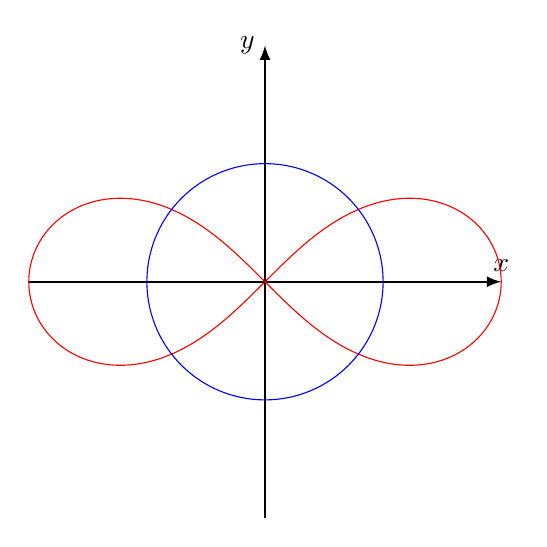
\begin{tikzpicture}
                \draw[thick,->,>=latex] (-3,0)--(3,0) node[above] {$x$};
                \draw[thick,->,>=latex] (0,-3)--(0,3) node[left] {$y$};
                \draw[red, domain=-45:45,scale=1.5,samples=500] plot (\x:{sqrt(4*cos(2*\x))});
                \draw[red, domain=-45:45,scale=1.5,samples=500] plot (\x:{-sqrt(4*cos(2*\x))});
                \draw[blue, domain=0:360,scale=1.5,samples=500] plot (\x:{1});
            \end{tikzpicture}
        \end{center}
        We first find the four points of intersection:
        \begin{equation}
            4\cos(2\theta)=1 \implies \cos (2\theta) = \frac{1}{4} \implies \theta = \pm 0.659
        \end{equation}
        or $\theta = \pi \pm 0.659$. Due to the symmetry, we only need to find the area of one half of the area we are interested in, which gives:
        \begin{align}
            \frac{1}{2}A &= \frac{1}{2}\int_{-0.659}^{0.659}(4\cos 2\theta - 1) \dd{\theta} \\ 
            &= \frac{1}{2}(2\sin 2\theta - \theta)\Big|^{0.659}_{-0.659} \\
            &= 1.277
        \end{align}
        so the area is $A=2.554$.
    \end{example}
    \item There are a few challenging examples:
    \begin{example}
        Suppose we wish to find the area between $r=\sin\theta$ and $r=\cos \theta$:
        \begin{center}
            \begin{tikzpicture}
                \draw[thick,->,>=latex] (-3,0)--(3,0) node[above] {$x$};
                \draw[thick,->,>=latex] (0,-3)--(0,3) node[left] {$y$};
                \draw[red, domain=0:360,scale=2.5,samples=500] plot (\x:{cos(\x)});
                \draw[blue, domain=0:360,scale=2.5,samples=500] plot (\x:{sin(\x)});
            \end{tikzpicture}
        \end{center}
        We know from symmetry that the intersection is at $\theta = \frac{\pi}{4}$. We notice that the contribution to the area from each curve $\rho$ is equal and \textit{independent} from each other. Therefore:
        \begin{equation}
            A = A_1 + A_2 = \int_0^{\pi/4} \frac{1}{2}\sin^2\theta \dd{\theta} + \int_{\pi/4}^{\pi/2} \frac{1}{2}\cos^2\theta \dd{\theta} = \frac{\pi}{8} - \frac{1}{4}
        \end{equation}
    \end{example}
    \item We can determine the arclength by working in parametric form. Let $x = r(\theta) \cos\theta$ and $y = r(\theta) \sin\theta$. Therefore:
    \begin{align}
        s &= \int_{\alpha}^{\beta} \sqrt{\left(\frac{dx}{d\theta}\right)^2 + \left(\frac{dy}{d\theta}\right)^2}\dd{\theta} \\ 
        &= \int_\alpha^\beta \sqrt{(r'\cos\theta - r\sin\theta)^2 + (r'\sin\theta + r\cos\theta)^2} \dd{\theta} \\ 
        &= \int_\alpha^\beta \sqrt{(r'^2\cos^2\theta + r^2\sin^2\theta - \cancel{2rr'\cos\theta\sin\theta}) + (r'^2\sin^2\theta + r^2\cos^2\theta + \cancel{2r'r\cos\theta\sin\theta})} \dd{\theta} \\ 
        &= \int_\alpha^\beta \sqrt{r^2(\cos^2\theta+\sin^2\theta) + r'^2(\cos^2\theta+\sin^2\theta)} \\ 
        &= \int_\alpha^\beta \sqrt{r^2 + \left(\frac{dr}{d\theta}\right)^2} \dd{\theta}
    \end{align}
    \begin{example}
        Suppose we want to find the arclength of $r=a(1-\cos\theta)$ from $0 \le \theta < 2\pi$. This looks like:
        \begin{center}
            \begin{tikzpicture}
                \draw[thick,->,>=latex] (-3,0)--(3,0) node[above] {$x$};
                \draw[thick,->,>=latex] (0,-3)--(0,3) node[left] {$y$};
                \draw[domain=0:360,scale=1.5,samples=500] plot (\x:{1-cos(\x)});
            \end{tikzpicture}
        \end{center}
        We have:
        \begin{align}
            s &= \int_0^{2\pi}\sqrt{r^2 + (r')^2} \dd{\theta} \\ 
            &= \int_0^{2\pi}\sqrt{a^2(1-2\cos\theta+\cos^2\theta)+a^2\sin^2\theta}\dd{\theta} \\ 
            &= a\int_0^{2\pi}\sqrt{2-2\cos\theta}\dd{\theta} \\ 
            &= a \int_0^{2\pi} \sqrt{4\sin^2\left(\frac{\theta}{2}\right)} \dd{\theta} \\ 
            &= 2a\left[-2\cos\left(\frac{\theta}{2}\right)\right]\Biggr|^{2\pi}_0 \\ 
            &= 8a
        \end{align}
    \end{example}
\end{itemize}
\end{document}

